\section{Study of transparent boundary conditions}
\label{sec:TBC}

\subsection{Introduction and motivational examples}

\indent The work presented in this section is an introduction to the objectives that we are looking for in this project, concerning the study of Transparent Boundary Conditions (TBCs). It was developed on the KdV equation, because, among the models studied and implement until here (KdV, BBM and Serre equations), it was the one for which we have obtained the best computational implementation.

\indent The TBCs are constructed such that the solution computed in the finite computational domain $\Omega$ coincides with the solution of the whole-space problem, restricted to $\Omega$ . In general, these boundary conditions are nonlocal in time,  so they must be approximated for an efficient numerical implementation \cite{Xavieretal2008}. Before moving to the models of wave propagation, in order to see in practice this definition we will implement a simple example, with analytical solution and TBCs, derived following \cite{Japhet2003}.  We will consider the 1D problem 

\begin{equation}
\begin{cases}
-u''(x) = 1 \ \ in \ \ \Omega = [0,2]\\
u(0) = 0 \\
u(2) = 0
\end{cases}
\end{equation}

\noindent whose solution is

$$u(x) = -\frac{x^2}{2} + x$$

\noindent and, considering the partition of $\Omega$ in $\Omega_1 = [0,1]$ and $\Omega_2 = [1,2]$, we will solve the problem

\begin{equation}
\begin{cases}
-u_1''(x) = 1 \ \ in \ \ \Omega_1\\
u_1(0) = 0 \\
B(u_1) = 0 \ \ at \ \ \Gamma=\{1\}
\end{cases}
\end{equation}

\noindent where the transparent boundary condition $B(u)$ is such that $u|_{\Omega_1} = u_1$.

\indent The TBC is written in the form $B(u) = \frac{\partial}{\partial x}u + D2N(u)$, where the D2N (Dirichlet to Neumann) operator is defined by

$$\left. D2N : \alpha(x) \mapsto \frac{\partial}{\partial x}v \right\rvert_\Gamma$$

\noindent where $\alpha$ is defined in the boundary $\Gamma$. In the case treated here, $\Gamma$ is a point, and therefore $\alpha$ is a scalar.

\indent The function $v$ is solution of

\begin{equation}
\begin{cases}
-v''(x) = 1 \ \ in \ \ \Omega_2\\
v(2) = 0 \\
v(1) = \alpha \ \ at \ \ \Gamma=\{1\}
\end{cases}
\end{equation}

\noindent so

$$v(x) = -\frac{x^2}{2} + \left(\frac{3}{2} - \alpha \right) + 2\alpha -1$$

\noindent and 

$$\left. \frac{\partial}{\partial x}v \right\rvert_{x=1} = \frac{1}{2} - \alpha$$

\indent Finally, the TBC reads

$$B(u_1) = \frac{\partial}{\partial x}u_1 + D2N(u_1) = \frac{\partial}{\partial x}u_1+ \frac{1}{2} - u_1$$

\indent The problem was solved with a finite difference method, with centered second-order approximation for the spatial derivative, for two different grids. The figure \ref{fig:TBClaplace} shows that the constructed TBC effectively provides a convergent solution.

\begin{center}
	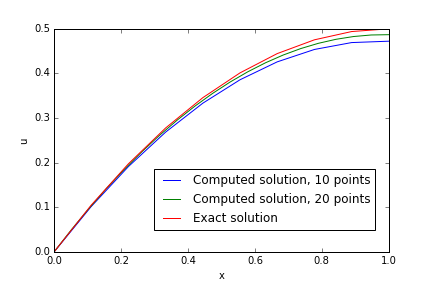
\includegraphics[scale=.5]{figures/TBClaplace.png}
	\captionof{figure}{Solutions for the Laplace equation with TBC \label{fig:TBClaplace}}
\end{center}

\indent Coming back to the wave models, we recall that, in the first simulations with the splitting method adopted to the resolution of the KdV equation, we did not make a rigorous application of appropriate boundary conditions. In fact, our initial objective was to validate the method; therefore, imposing periodic or homogeneous Dirichlet and Neumann conditions, we analyzed the evolution of the solution only before the arrival of the wave to the boundaries.

\indent The following example shows very clearly the influence of inappropriate boundary conditions on the solution. We solved two times the same problem, with the same initial solution, boundary conditions, and spatial and time discretizations: 

\begin{equation}
    \begin{cases}
    u_t + u_x + (u^2)_x + u_{xxx} = 0 \ , \ \ x \in \Omega=[a,b] \ \ t \in [0, t_{max}] \\
    u(x,0) = \Phi(x) \\
    u(a,t) = 0 \\
    u(b,t) = 0 \\
    u_x(b,t) = 0  \\ 
    \end{cases}
\end{equation}

\indent The only difference is the size of the domain of each problem : they were chosen such that the wave reaches the boundaries (within the maximal time of simulation) in the first problem, but not in the second. The difference between the solution increases with the time, beginning in the boundary and propagating to the whole domain :

\begin{figure}[h]
	\begin{subfigure}{.3\linewidth}
		\center
		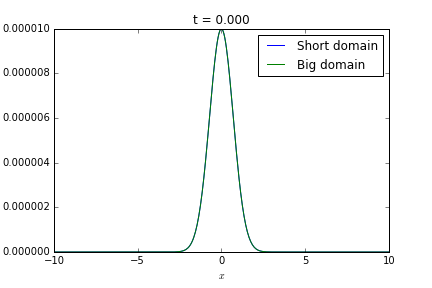
\includegraphics[scale=.3]{figures/motivational1A.png}	
	\end{subfigure}
	\begin{subfigure}{.3\linewidth}
		\center
		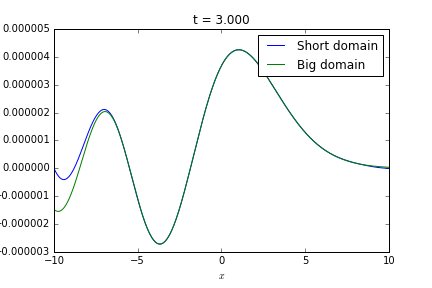
\includegraphics[scale=.3]{figures/motivational1B.png}	
	\end{subfigure}
	\begin{subfigure}{.3\linewidth}
		\center
		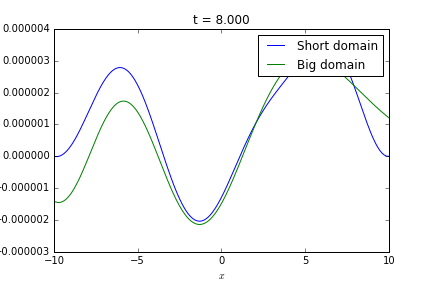
\includegraphics[scale=.3]{figures/motivational1C.png}	
	\end{subfigure}
	\caption{First motivational example : comparison between the solutions in a small and a big domain}
\end{figure}

\indent Therefore, we look for boundaries conditions that can efficiently simulate the called Transparent Boundary Conditions (TBCs), i.e., in a such a way that the solution calculated in the computational domain $\Omega$ coincides with solution of the whole-space restricted to $\Omega$. As a consequence, we want the boundaries not to have an influence on the solution, so, when the wave reaches the boundary, it will simply "exit" the domain. The following example shows another motivation for this work.

\indent We want to solve the following problem :

\begin{equation}
    (P_1) \begin{cases}
    u_t + u_x + (u^2)_x + u_{xxx} = 0 \ , \ \ x \in \Omega_1 = [0,L], \ \ t \in [0, t_{max}] \\
    u(x,0) = \Phi(x) \\
    u(0,t) = 0 \\
    u_x(0,t) = 0 \\
    u(L,t) = g(t)  \\ 
    \end{cases}
\end{equation}

\indent We seek a function $g(t)$ to simulate the TBC. In order to do this, we will solve before the problem

\begin{equation}
    (P_2) \begin{cases}
    u_t + u_x + (u^2)_x + u_{xxx} = 0 \ , \ \ x \in \Omega_2 = [0,2L], \ \ t \in [0, t_{max}] \\
    u(x,0) = \Phi(x) \\
    u(0,t) = 0 \\
    u_x(0,t) = 0 \\
    u(2L,t) = 0  \\ 
    \end{cases}
\end{equation}

\noindent and we impose $g(t) = u_2(t)$, where $u_2$ is the solution of $(P_2)$. To obtain more precise results, the two computations are made with the same mesh size and time step.

\indent Suppose that there is a unique solution $u_1$ to $(P_1)$. We can easily see that $u_2|_{\Omega_1}$ is also a solution of $(P_1)$. Therefore, $u_1 = u_2|_{\Omega_1}$. It justifies why our procedure works as a TBC, as shown in the figure \ref{fig:motivation2} (close-up in the region close to the right boundary) :

\begin{figure}[h]
	\begin{subfigure}{.5\linewidth}
		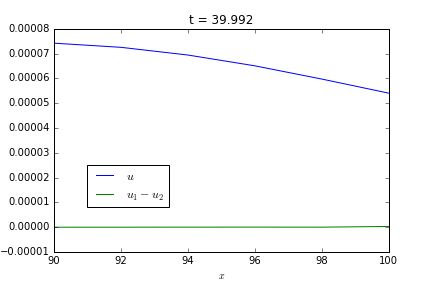
\includegraphics[scale=.5]{figures/motivational2A.png}	
	\end{subfigure}
	\begin{subfigure}{.5\linewidth}
		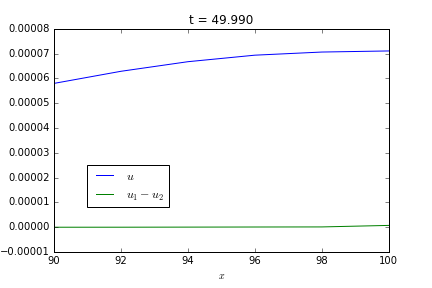
\includegraphics[scale=.5]{figures/motivational2B.png}	
	\end{subfigure}
	\caption{Second motivational example : solution with an "exact" Dirichlet condition at the right boundary \label{fig:motivation2}}
\end{figure}

\subsection{Optimization of Robin boundary conditions to simulate TBCs}

\subsubsection{Robin boundary conditions up to the first derivative}

\indent Although the motivating result presented in the above example, we cannot apply this procedure in practice. In fact, computing the solution in a larger domain and using it as exact solution is only a trick, which has no practical interest. Therefore, we want to determinate approximations for a TBC without having a referential solution. 

\indent The KdV will be solved in the domain $[-L,L]$ with the following boundary conditions (imposed in the resolution of the second equation of the split method):

\begin{equation}
\begin{cases}
    u(-L) = 0 \\
    u_x(-L) = 0 \\
    \alpha u(L) + \beta u_x(L) = 0,  \ \ \alpha,\beta > 0
\end{cases}
\end{equation}

\indent In the third condition, called a Robin boundary condition, the parameters $\alpha$ and $\beta$ (or, equivalently, the parameter $\beta/\alpha$) will be optimized in order to simulate a TBC. In a first moment, we will consider Robin BCs up to the first derivative of the solution.

\indent To find the optimal coefficients, we will test several pairs $(1,\beta/\alpha)$ (including the limits $\beta/\alpha \rightarrow 0$ and $\beta/\alpha \rightarrow \infty$, corresponding respectively to Dirichlet and Neumann BCs) and compute the error regarding to a referential solution $u_{ref}$, computed in a domain $[-2L,2L]$. Two errors will be computed, for each time step $t_n$ :

\begin{equation}
e_1^n = \sqrt{\sum_{i=0}^N{\left( u^n_i - (u_{ref})^n_i\right)^2}} 
\end{equation}

\begin{equation}
e_2^n =  u^n_N - (u_{ref})^n_N
\end{equation}

\indent $e_2^n$ is computed in order to show that most part of the error $e_1^n$ of the entire domain occurs in the boundary.

\indent The figures \ref{fig:robin1} to \ref{fig:robinErrorsExample} show some snapshots and the evolution of $e_1$ and $e_2$ for some values of $\beta/\alpha$ . The figure \ref{fig:robinErrorsAll} compares $e_2$ for many other values, including the pure Dirichlet (with $\alpha = 1, \beta = 0$, so $log(\beta/\alpha) = -\infty$) and pure Neumann (with $\alpha = 0, \beta = 1$, with $\beta/\alpha$ computationally represented by  $10^{10}$)  conditions.


\begin{figure}[h]
	\begin{subfigure}{.5\linewidth}
		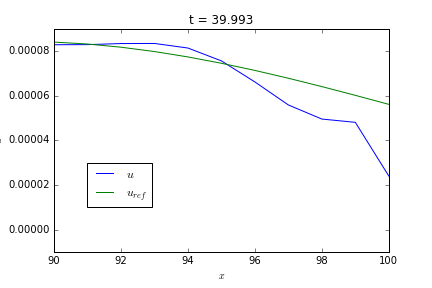
\includegraphics[scale=.5]{figures/robin1A.png}	
	\end{subfigure}
	\begin{subfigure}{.5\linewidth}
		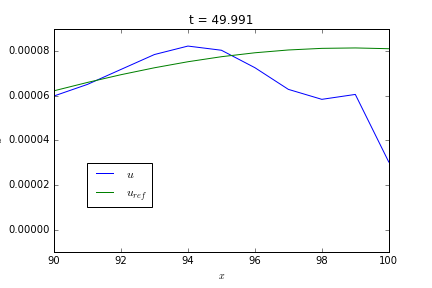
\includegraphics[scale=.5]{figures/robin1B.png}	
	\end{subfigure}
	\caption{Computed and the referential solution for  $\beta/\alpha = 1$ \label{fig:robin1}}
\end{figure}

\noindent\begin{minipage}{\textwidth} 
	\begin{minipage}{.5\textwidth} 
		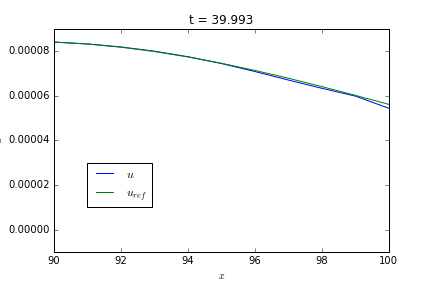
\includegraphics[scale=.5]{figures/robin10A.png}	
	\end{minipage}
	\begin{minipage}{.5\linewidth}
		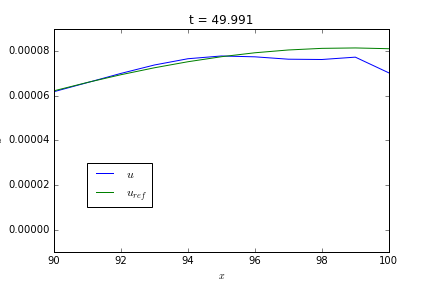
\includegraphics[scale=.5]{figures/robin10B.png}	
	\end{minipage}
	\captionof{figure}{Computed and the referential solution for  $\beta/\alpha = 10$ \label{fig:robin10}}
\end{minipage}

\noindent\begin{minipage}{\textwidth} 
	\begin{minipage}{.5\textwidth} 
		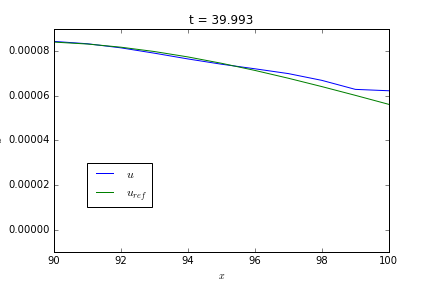
\includegraphics[scale=.5]{figures/robin100A.png}	
	\end{minipage}
	\begin{minipage}{.5\linewidth}
		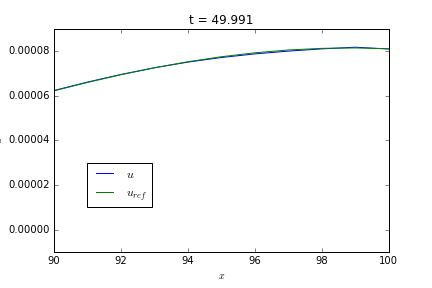
\includegraphics[scale=.5]{figures/robin100B.png}	
	\end{minipage}
	\captionof{figure}{Computed and the referential solution for  $\beta/\alpha = 100$ \label{fig:robin100}}
\end{minipage}

\noindent\begin{minipage}{\textwidth} 
	\begin{minipage}{.3\textwidth} 
		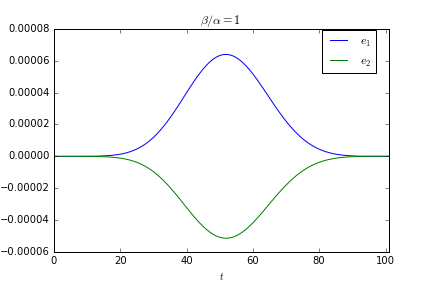
\includegraphics[scale=.3]{figures/robin1Error.png}	
		\captionof{subfigure}{$\beta/\alpha = 1$}
	\end{minipage}
	\begin{minipage}{.3\textwidth} 
		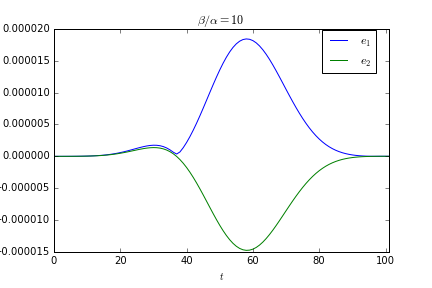
\includegraphics[scale=.3]{figures/robin10Error.png}	
		\captionof{subfigure}{$\beta/\alpha = 10$}
	\end{minipage}
	\begin{minipage}{.3\textwidth}
		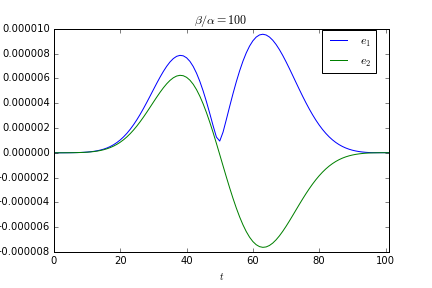
\includegraphics[scale=.3]{figures/robin100Error.png}	
		\captionof{subfigure}{$\beta/\alpha = 100$}
	\end{minipage}
	\captionof{figure}{Errors between the computed and the referential solution \label{fig:robinErrorsExample}}
\end{minipage}

\begin{center}
		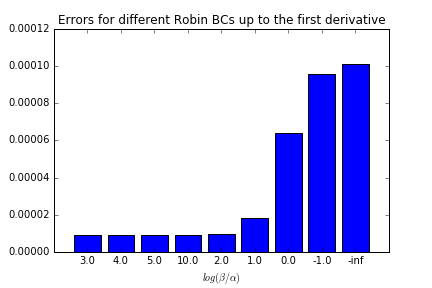
\includegraphics[scale=.6]{figures/robinErrors1.png}
	     \captionof{figure}{Error $||e_1| = \sum_{n=0}^{n_{max}}(e^n_1)^2$ between the computed and the referential solution for many values of $\beta/\alpha$ \label{fig:robinErrorsAll}}
\end{center}


\indent The results presented in the figures \ref{fig:robin1} to \ref{fig:robinErrorsAll} show that boundary conditions with stronger Neumann character produce better approximations to the TBC, compared to more Dirichlet-type conditions. The results for pure Neumann conditions and for Neumann with a small but non-zero Dirichlet were very close. In fact, setting the solution to zero in the boundary is a too much strong condition, and the Neumann condition captures in a more satisfactory way the smoothness of the propagating wave.

\subsubsection{Robin boundary conditions up to the second derivative}

\indent We repeated the tests described above, but replacing the boundary condition in the right boundary by $\alpha u(L) + \beta u_x(L) + \gamma u_{xx}(L) = 0,  \ \ \alpha,\beta, \gamma > 0$.

\indent The values of $\alpha$ and $\beta$ will be fixed and equal to the ones that gave the minimal error in the previous simulations ($(\alpha,\beta) = (1,1000)$). We will show directly the graph containing the errors for many values of $\gamma/\beta$ (figure \ref{fig:robinErrorsAll2}, which should be compared with the figure \ref{fig:robinErrorsAll}. Similarly to the previous conclusions, we observe a better approximation of the TBCs for stronger values of $\gamma/\beta$.

\begin{center}
		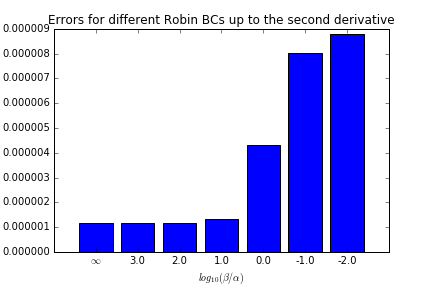
\includegraphics[scale=.6]{figures/robinErrors2.png}
	     \captionof{figure}{Error $||e_1| = \sum_{n=0}^{n_{max}}(e^n_1)^2$between the computed and the referential solution for many values of $\gamma/\beta$, with Robin conditions up to the second derivative \label{fig:robinErrorsAll2}}
\end{center}
